\documentclass[crop,tikz]{standalone}

\usetikzlibrary{angles}

\begin{document}
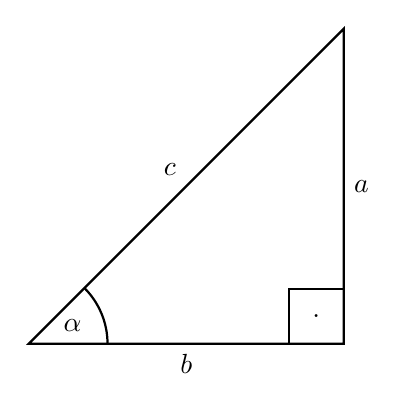
\begin{tikzpicture}[thick]
  \draw (0,0) coordinate (a) -- node[below] {$b$}
        (4,0) coordinate (c) -- node[right] {$a$}
        (4,4) coordinate (b) -- node[above left] {$c$} cycle;
  \pic[draw, angle eccentricity=0.6, angle radius=1cm, pic text={$\alpha$}] {angle = c--a--b};
  \pic[draw, angle eccentricity=0.5, angle radius=0.7cm, pic text=.] {right angle = b--c--a};
\end{tikzpicture}
\end{document}
